\chapter{Introduction}
\label{chap:introduction}

In recent years, the deployment of applications has increasingly relied on cloud-based resources. Prominent cloud service providers such as Google Cloud~\cite{googlecloud}, Amazon Web Services (AWS)~\cite{aws}, and Microsoft Azure~\cite{azure} have established expansive data centers to meet the growing demand for computational and storage capabilities. These data centers consist of extensive server infrastructures, where each server is equipped with essential resources such as compute power and memory. Applications request these resources on demand, and providers bill clients based on the volume and duration of resource usage~\cite{cloud1, cloud2, cloud3}.

However, despite the flexibility of cloud computing, a significant challenge persists in resource utilization within cloud data centers. Specifically, the tight coupling of compute and memory resources in individual servers often results in inefficient resource allocation, leading to underutilization and waste~\cite{cxl_azure, tpp, pond,legoos}. This problem becomes particularly apparent when applications request resources that do not align well with the available capacity of individual servers. Even when there is sufficient total capacity across multiple servers, the rigid allocation of resources within each server can lead to unused compute or memory, hindering overall system efficiency.

The growing demand for scalable and efficient data center architectures has led to the emergence of resource disaggregation~\cite{mind, legoos, disagg, memdisagg1, memdisagg2, memdisagg3, memdisagg4, memdisagg5, memdisagg6}. This modern paradigm represents a significant shift from traditional monolithic server architectures. In conventional setups, servers are typically equipped with a fixed combination of compute, memory, and storage resources. In contrast, resource-disaggregated systems physically separate these resources and distribute them across various interconnects, such as networks~\cite{disagg, legoos, mind}, Compute Express Link (CXL)~\cite{cxl, cxlasic}, and others. This separation allows for more flexible resource allocation and utilization, providing a promising solution to the resource inefficiency issues seen in traditional architectures.




\section{Memory Disaggregation}

Within the broader context of resource disaggregation in modern data center architectures, \textbf{memory disaggregation}~\cite{memdisagg1, memdisagg2, memdisagg3, memdisagg4, memdisagg5, memdisagg6} plays a crucial and foundational role. In traditional monolithic architecture, memory often becomes a bottleneck, limiting the scalability and adaptability of applications. This issue has been frequently observed and reported in production data centers~\cite{memory1, memory2, memory3, memory4, memory5, memory6, memory7, memory8, memory9, memory10}. By decoupling memory resources from compute and storage elements and presenting them as pooled, disaggregated resources~\cite{pool1, pool2}, data centers can achieve increased efficiency, scalability, and adaptability. Memory-intensive applications~\cite{redis, ramcloud, sparkmemory} can access the memory they need on demand, without being constrained by the limitations of individual servers. 

Memory disaggregation has emerged as a viable solution to this problem. By decoupling compute and memory resources within a rack-scale server and creating independent resource pools connected through high-speed interconnects such as CXL or Ethernet, cloud providers can allocate memory more flexibly, improving overall utilization rates. This approach holds the potential to significantly reduce waste, optimize performance, and lower operational costs by enabling more granular and efficient allocation of memory.

\begin{figure}[t]
    \centering
    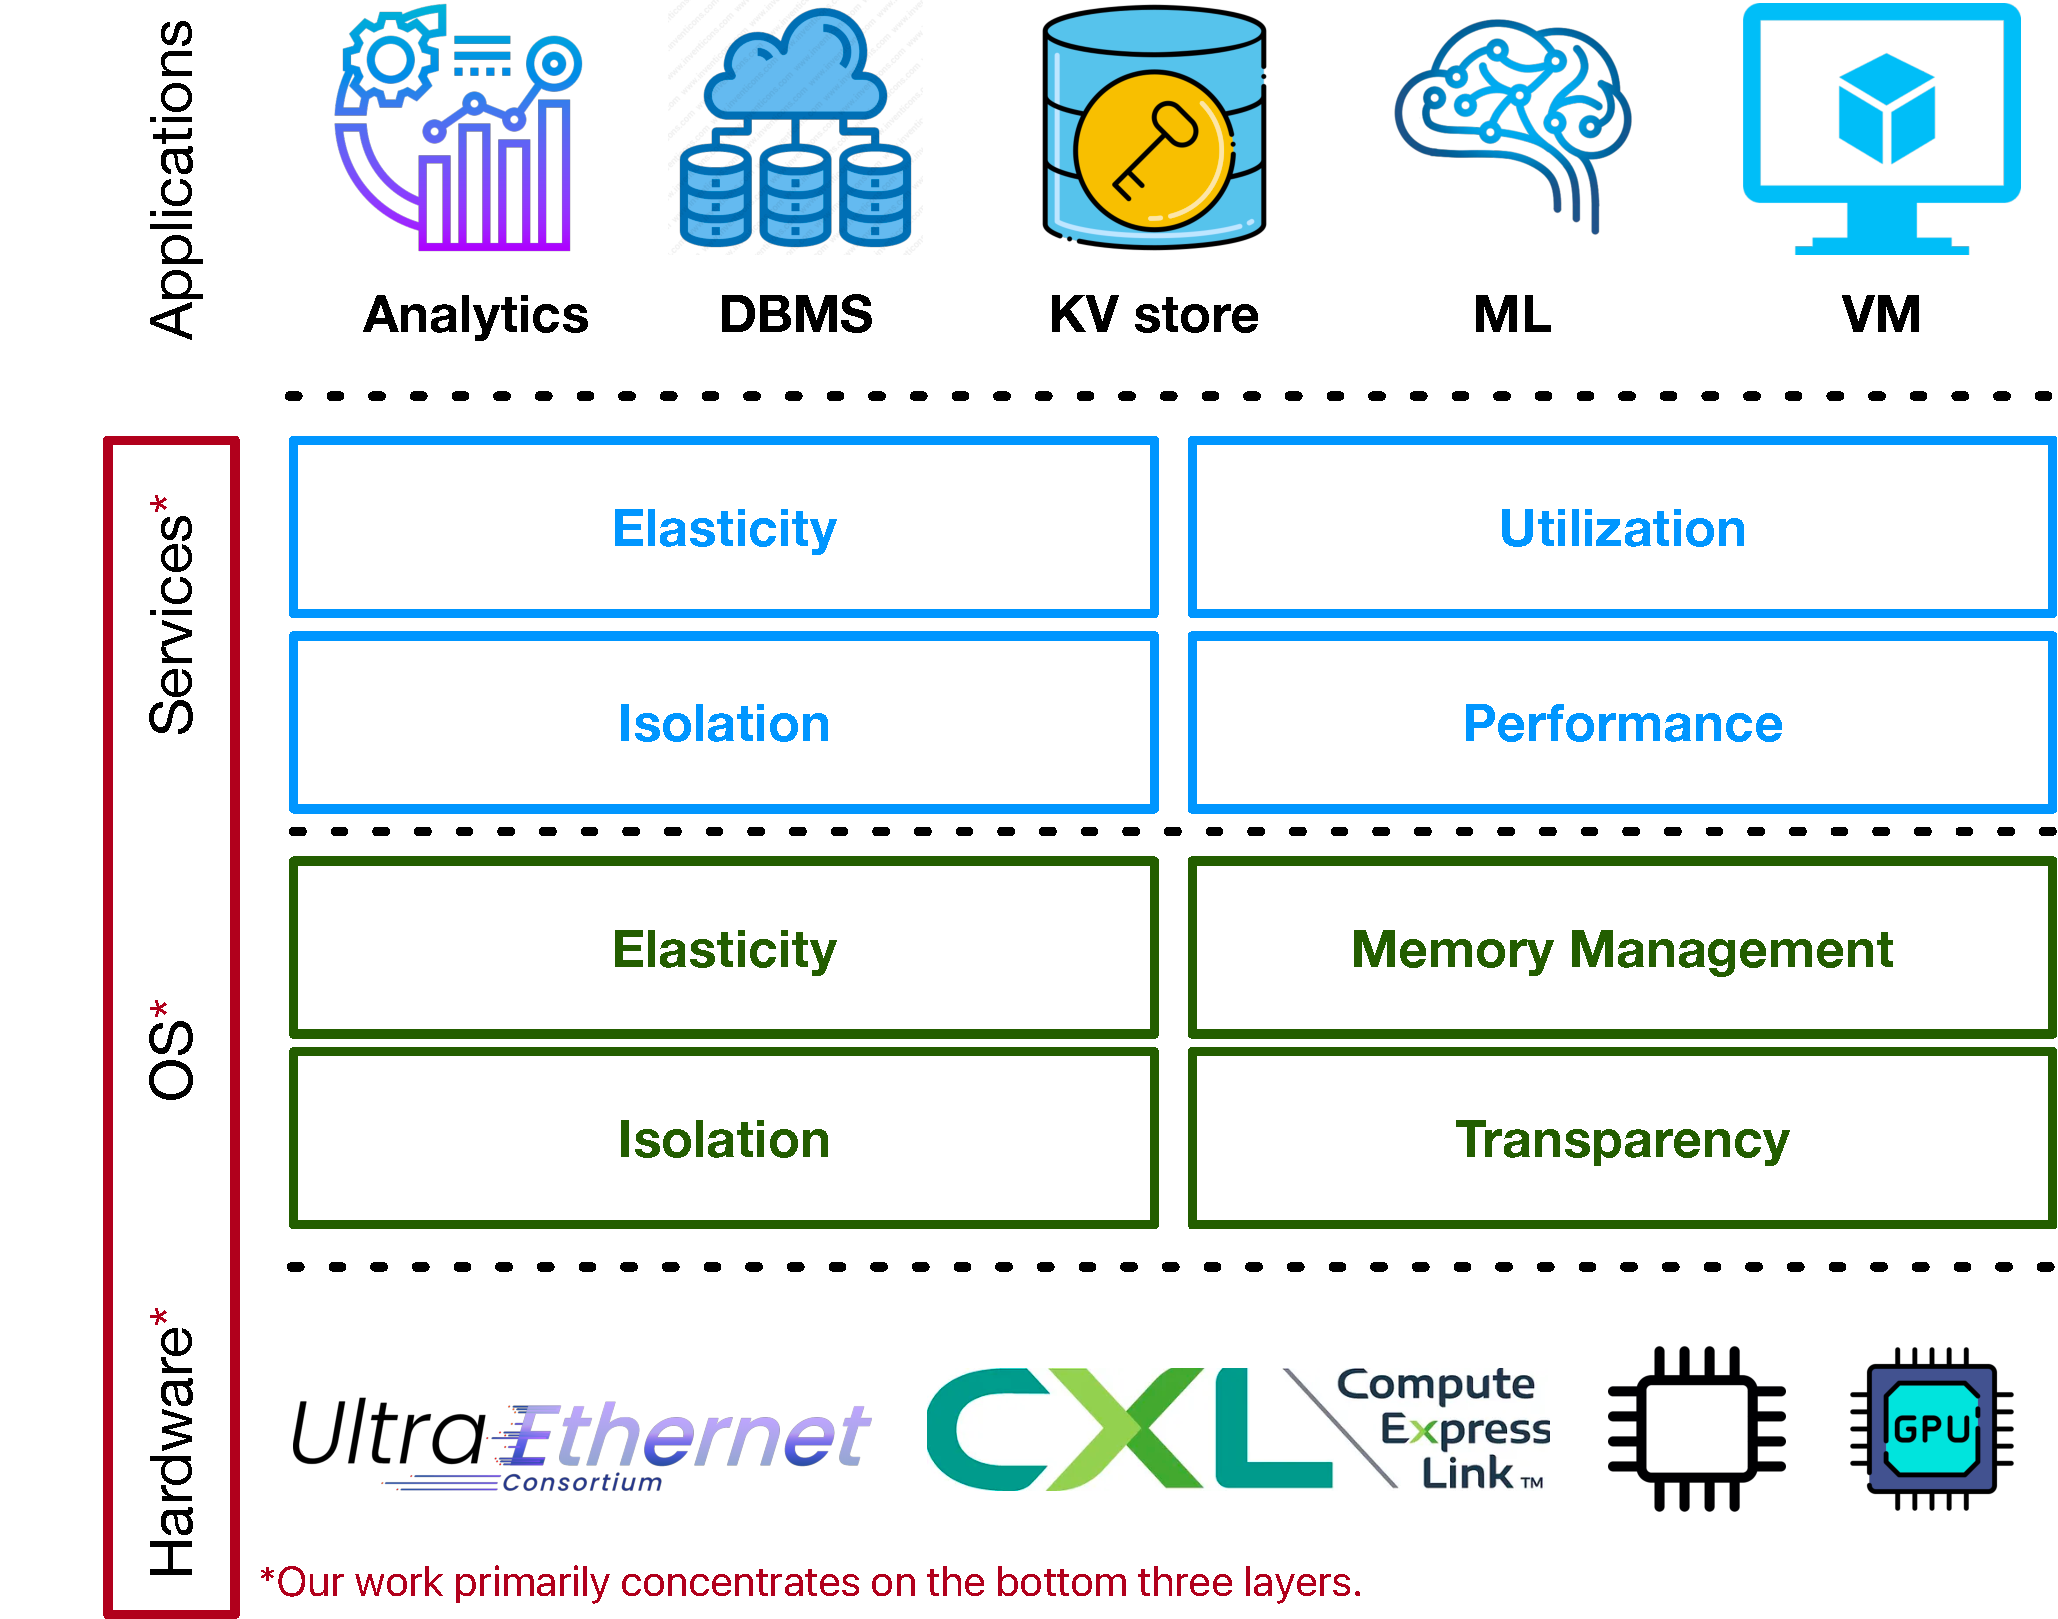
\includegraphics[width=0.7\columnwidth]{stack.pdf}
      \caption[Cloud Stack of Disaggregated Architecture]{\textbf{Cloud Stack of Disaggregated Architecture.} The service layer offers a specialized memory management interface tailored to specific application needs, as discussed in Chapter~\ref{chap:service}. In contrast, the OS layer provides a more generic interface, prioritizing transparency to ensure applications can run without modification and without requiring awareness of underlying hardware details.} 
      \label{fig:stack}
\end{figure}


\section{Cloud Provider and Application Requirements}

Cloud vendors are eager to adopt memory disaggregation to improve scalability and reduce costs by optimizing resource utilization~\cite{pond, tpp}. By decoupling memory from compute nodes, disaggregation allows for more flexible resource management, enabling cloud providers to pool and allocate memory across applications based on demand. However, achieving this requires smart allocation and resource management strategies. For instance, without intelligent allocation, memory could be under-utilized or over-provisioned, leading to inefficiencies in cloud data centers. Therefore, cloud providers need solutions that can dynamically manage resources to maximize overall efficiency.

From the perspective of users, however, adopting disaggregated memory presents additional concerns. Developers are typically reluctant to re-implement or modify application code just because the underlying hardware has shifted to a disaggregated architecture. They need a system that provides \textbf{transparency}, ensuring that applications can leverage disaggregated memory without extensive rewrites or optimizations, thus reducing development overhead.

Moreover, performance is a critical factor for users, particularly for latency-sensitive applications. Disaggregated architectures introduce slower interconnects like Ethernet, which can increase the time it takes to access memory compared to traditional local memory setups. For many applications, this added latency can lead to unacceptable slowdowns. Thus, ensuring \textbf{good application performance} despite the complexities of remote memory access is essential, especially for workloads that demand low-latency responses~\cite{mind, chase}.

In summary, for disaggregation to be viable and widely adopted, cloud providers must meet three key requirements:

\textbf{R1: Achieving Transparency} — Applications should be able to utilize disaggregated memory without requiring significant modifications or re-implementation. Transparency is crucial to ensure seamless adoption and minimize the burden on developers.

\textbf{R2: Ensuring Good Application Performance} — Performance must remain high, even when accessing memory over slower interconnects. Latency-sensitive applications should not experience significant degradation in performance when running on disaggregated systems.

\textbf{R3: Optimizing Resource Utilization} — Cloud providers must efficiently allocate and manage memory and compute resources across applications to avoid under-utilization or over-provisioning, thereby maximizing system efficiency and reducing costs.


\section{Challenges in Disaggregated Memory Architectures}

Despite the clear requirements for memory disaggregation, several challenges make it difficult to meet all of these goals simultaneously. The current cloud stack, designed for monolithic architectures, introduces inherent limitations when applied to disaggregated systems. These challenges can be grouped into three main categories:

\paragraphb{C1: Inefficient Resource Multiplexing in Disaggregated Memory Systems}

To optimize resource utilization, memory resources must be shared efficiently across multiple applications in a disaggregated architecture. However, unlike traditional systems where memory is tightly coupled to compute nodes, disaggregated architectures require memory to be dynamically multiplexed between multiple nodes. This introduces the risk of both under-utilization and over-provisioning, which can degrade overall system performance~\cite{jiffy, pocket}. Additionally, memory isolation becomes a concern when resources are shared across applications, and managing memory lifetime and garbage collection in a shared environment adds further complexity. These issues directly challenge the goal of optimizing resource utilization.

\paragraphb{C2: High-Latency Memory Access in Disaggregated Architectures}

To achieve good application performance, disaggregated memory systems must minimize the performance impact of accessing remote memory. However, due to the inherent latency of networked memory, remote memory access is much slower than local memory. Latency-sensitive applications, which require fast and frequent memory access, are particularly vulnerable to this degradation in performance~\cite{mind, chase}. For example, accessing local DRAM typically takes under 200 nanoseconds~\cite{cxl1, cxl2}, while accessing memory over a network can take several microseconds~\cite{mind,infiniswap}. This gap in latency is a significant barrier to maintaining the performance required by modern cloud applications.

\paragraphb{C3: Different Performance Characteristics in Next-Generation Interconnects}

To achieve transparency, cloud providers need a unified service and OS layer that can manage resources across different interconnects without requiring extensive application re-implementation. However, next-generation interconnects like Compute Express Link (CXL) and traditional interconnects like Ethernet exhibit vastly different performance characteristics. Ethernet, with its packet-based communication, is not well-suited for fine-grained memory access, while CXL leverages memory semantics over PCIe links to provide lower-latency memory operations~\cite{cxl1, cxl2, demystify}. These differences complicate system management and make it difficult to abstract the underlying hardware in a way that provides transparency to applications, posing a significant challenge to R1.


\paragraphb{Summary} 

Addressing the challenges of disaggregated memory cannot be resolved by focusing on a single layer of the cloud stack. Instead, it requires careful hardware-software co-design and cross-layer optimizations. For example, improving interconnect technologies like CXL at the hardware level is crucial to minimizing latency, but this alone is insufficient without corresponding changes in the OS and service layers to manage memory allocation efficiently across varied performance characteristics. Similarly, tackling issues like memory isolation or garbage collection requires coordination between hardware (e.g., memory controllers) and software (e.g., OS memory managers) to ensure proper resource sharing and isolation. Without these coordinated efforts, the potential of disaggregated architectures could be undermined by inconsistent performance and inefficient utilization of resources across the stack


\section{Thesis Overview}

In this dissertation, we take a top-down approach to address the key challenges of disaggregated memory architectures by optimizing memory management across the Service, OS, and Hardware layers of the cloud stack. The core challenges, including inefficient resource multiplexing, high-latency memory access, and diverse performance characteristics of next-generation interconnects, are tackled through this layered approach.


\subsection{Elastic Memory Multiplexing in the Service Layer}

At the highest layer, we address the challenge of inefficient resource multiplexing by exploring how memory resources can be elastically shared across multiple applications. We propose \textit{Jiffy}, an end-to-end system design that provides memory management as a service, allowing applications to efficiently share a dynamic pool of memory. Jiffy solves the challenge of under-utilization and over-provisioning by offering elastic memory allocation and interfaces for common data structures, making it broadly applicable to cloud applications. This solution directly tackles C1 by optimizing memory utilization at the service layer, enabling multiple applications to share memory without sacrificing performance or efficiency.

\subsection{Near-memory Processing in the Operating System Layer}

In the OS layer, we address the challenge of high-latency memory access in disaggregated systems. Our goal is to enable applications to transparently utilize disaggregated memory without requiring modifications. Traditional OS designs struggle to manage memory that is decoupled across multiple nodes, leading to significant latency, especially for cache-unfriendly applications. To mitigate this, we introduce \textit{PULSE}, a near-memory accelerator specifically optimized for pointer traversal workloads. \textit{PULSE} reduces interconnect overhead by offloading memory-intensive tasks to near-memory processors, significantly improving performance for applications affected by high-latency memory access. This enhancement enables the system to efficiently support a broader range of workloads in disaggregated environments.

\subsection{Memory Management for Next-Gen Interconnects in the Hardware Layer}

At the hardware layer, we tackle the challenge of diverse performance characteristics of next-generation interconnects. As emerging technologies like CXL replace traditional interconnects like Ethernet, new memory management strategies are required to fully leverage these advancements. We evaluate CXL 1.1 extended memory in single-host environments and explore how disaggregated memory systems can benefit from its low-latency, high-bandwidth capabilities. By adapting memory management to support multiple tiers of memory efficiently across various applications, we address the variability in interconnect performance and ensure that cloud data centers can fully harness the potential of next-generation interconnects.

\section{Outline and Previously Published Work}

This dissertation is organized as follows. Chapter~\ref{chap:service} introduces Jiffy, a distributed memory management system that decouples memory capacity and lifetime from compute in the serverless paradigm. Chapter~\ref{chap:os} describes a innovated system design: PULSE, a framework centered on enhancing in-network optimizations for irregular memory accesses within disaggregated data centers. Chapter ~\ref{chap:hardware} presents our exploration in latest Compute Express Link(CXL) hardware. We conclude with our contributions and possible future work directions in Chapter~\ref{chap:future}.

Chapter~\ref{chap:service} revises material from~\cite{jiffy}\footnote{Work done in collaboration with Rachit Agarwal, Aditya Akella, and Ion Stoica}. Chapter~\ref{chap:os} revises material from~\cite{chase}\footnote{Work done in collaboration with Seung-seob Lee and Abhishek Bhattacharjee}. Finally, Chapter~\ref{chap:hardware} revises material from~\cite{cxleurosys}\footnote{Work done in collaboration with the Bytedance Infrastructure team}.
